\chapter{Manuel d'utilisation}

\subsection {Principe}
Deux joueurs doivent s'entraider pour faire avancer leur balle à travers
des niveaux. Pour cela les joueurs exploitent différents mécanismes
physiques.
\\

Le jeu est constitué de niveaux, chaque niveau
étant représentés par une grille de blocs en deux dimensions. Les blocs interagissent
avec les balles et la physique du jeu comme défini dans les sections \ref{OB}.
\\

Les joueurs valident un niveau en faisant parvenir leurs
balles sur un bloc d'arrivée. Ils terminent ainsi le niveau, le but étant de tous
les achever.

\subsection {Menu de sélection}

\subsubsection{Menu principal}

Au lancement du jeu le menu principal apparait :


\begin{figure} [h]
    \centerline {\includegraphics[width=13cm]{figures/menu_principale.png}}
    \caption {Menu principal}
    \label {fig:MP}
\end{figure}

\noindent Ce menu [\ref{fig:MP}] se compose de quatre boutons:\\
\begin {itemize}
\item \bf Le bouton jouer [\ref{fig:MJ}]\\
\end {itemize}

Il permet d'accéder au menu de sélection des niveaux


%\item règles du jeu : affiche les règles du jeu.
%\item Éditeur : permet de crée un nouveau niveau ou de modifier un niveau existant.
%\item Quitter : permet de quitter le jeu.\\

\newpage

\begin{figure} [!h]
    \centerline {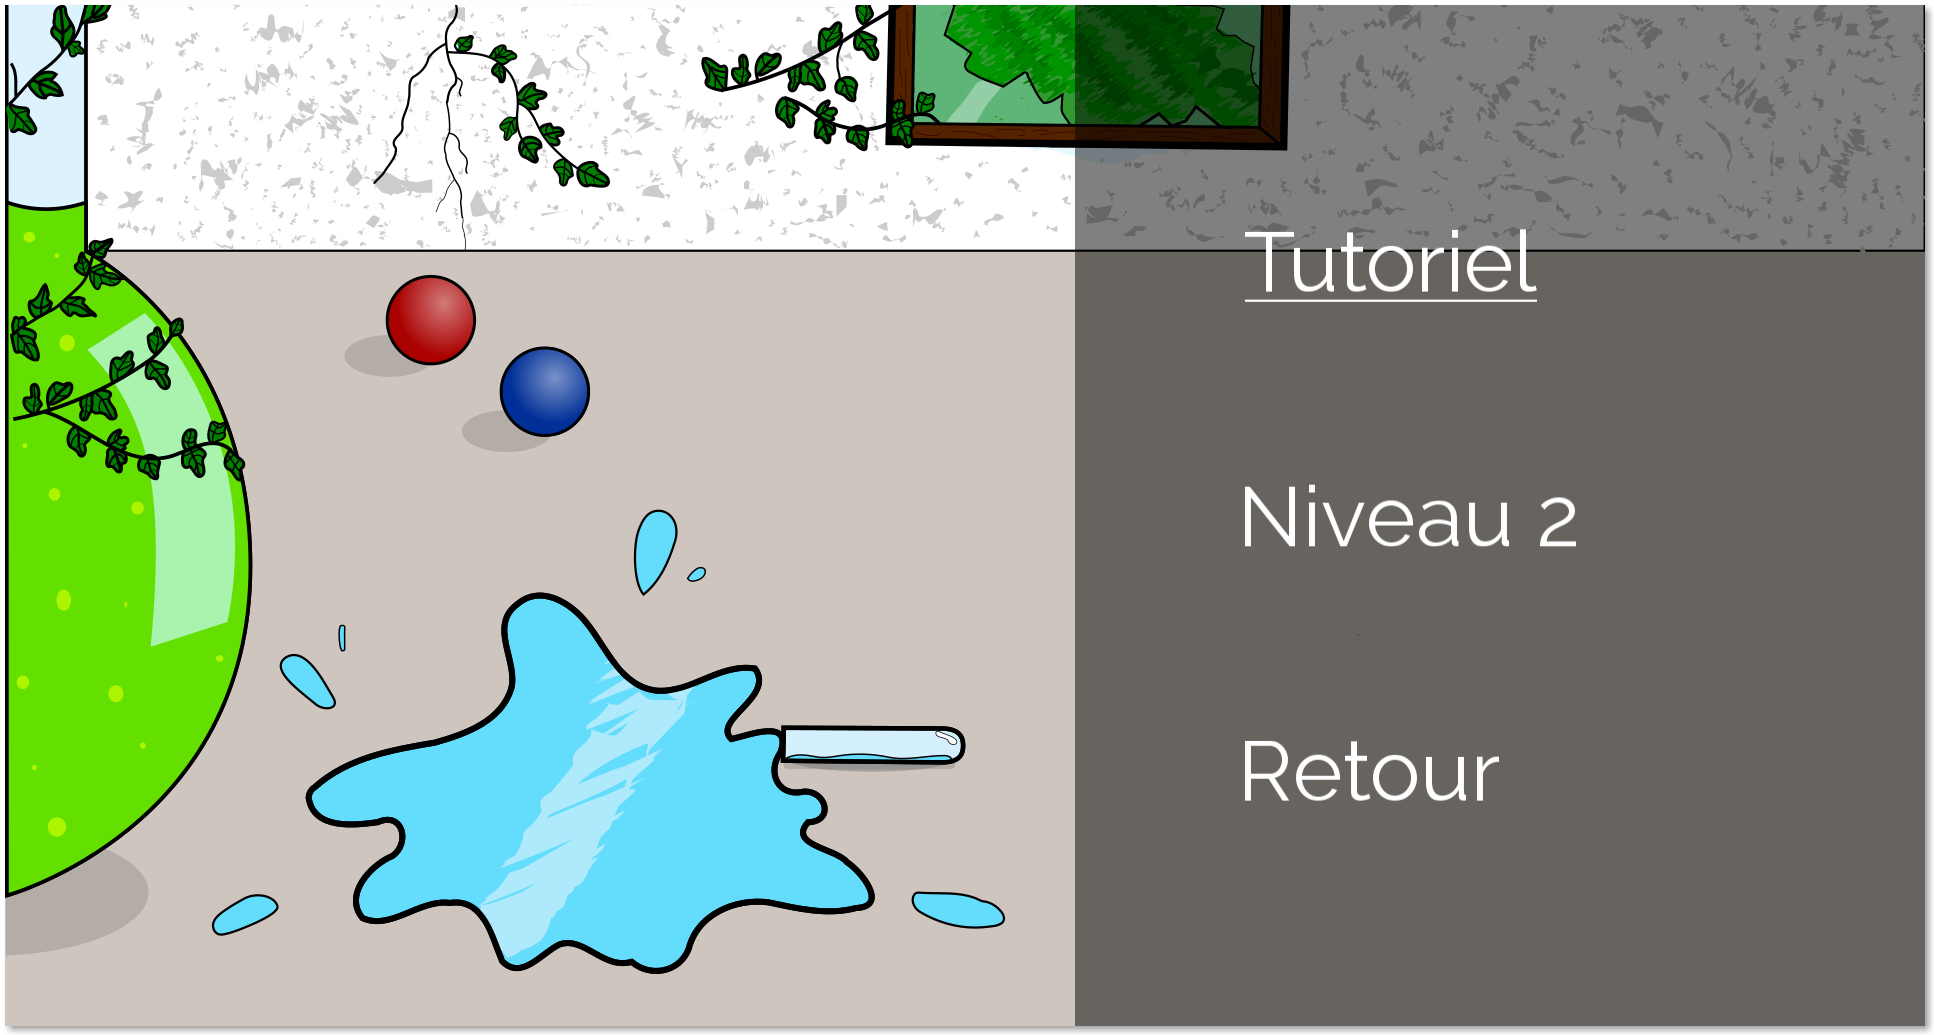
\includegraphics[width=13cm]{figures/menu_jouer.png}}
    \caption {Menu jouer}
    \label {fig:MJ}
\end{figure}

\noindent Ce menu [\ref{fig:MJ}] se compose de deux types de boutons : les boutons niveaux permettent aux joueurs de choisir un espace de jeu et
le bouton retour de revenir vers le menu principal [\ref{fig:MP}].\\

\begin {itemize}
\item \bf Le bouton règles du jeu.
\end {itemize}

Ce bouton affiche les règles du jeu.
\\
\\

\begin {itemize}
\item \bf Le bouton éditeur.
\end {itemize}

Ce bouton permet de créer un nouveau niveau ou de modifier un niveau existant.

\newpage

\begin{figure} [!h]
    \centerline {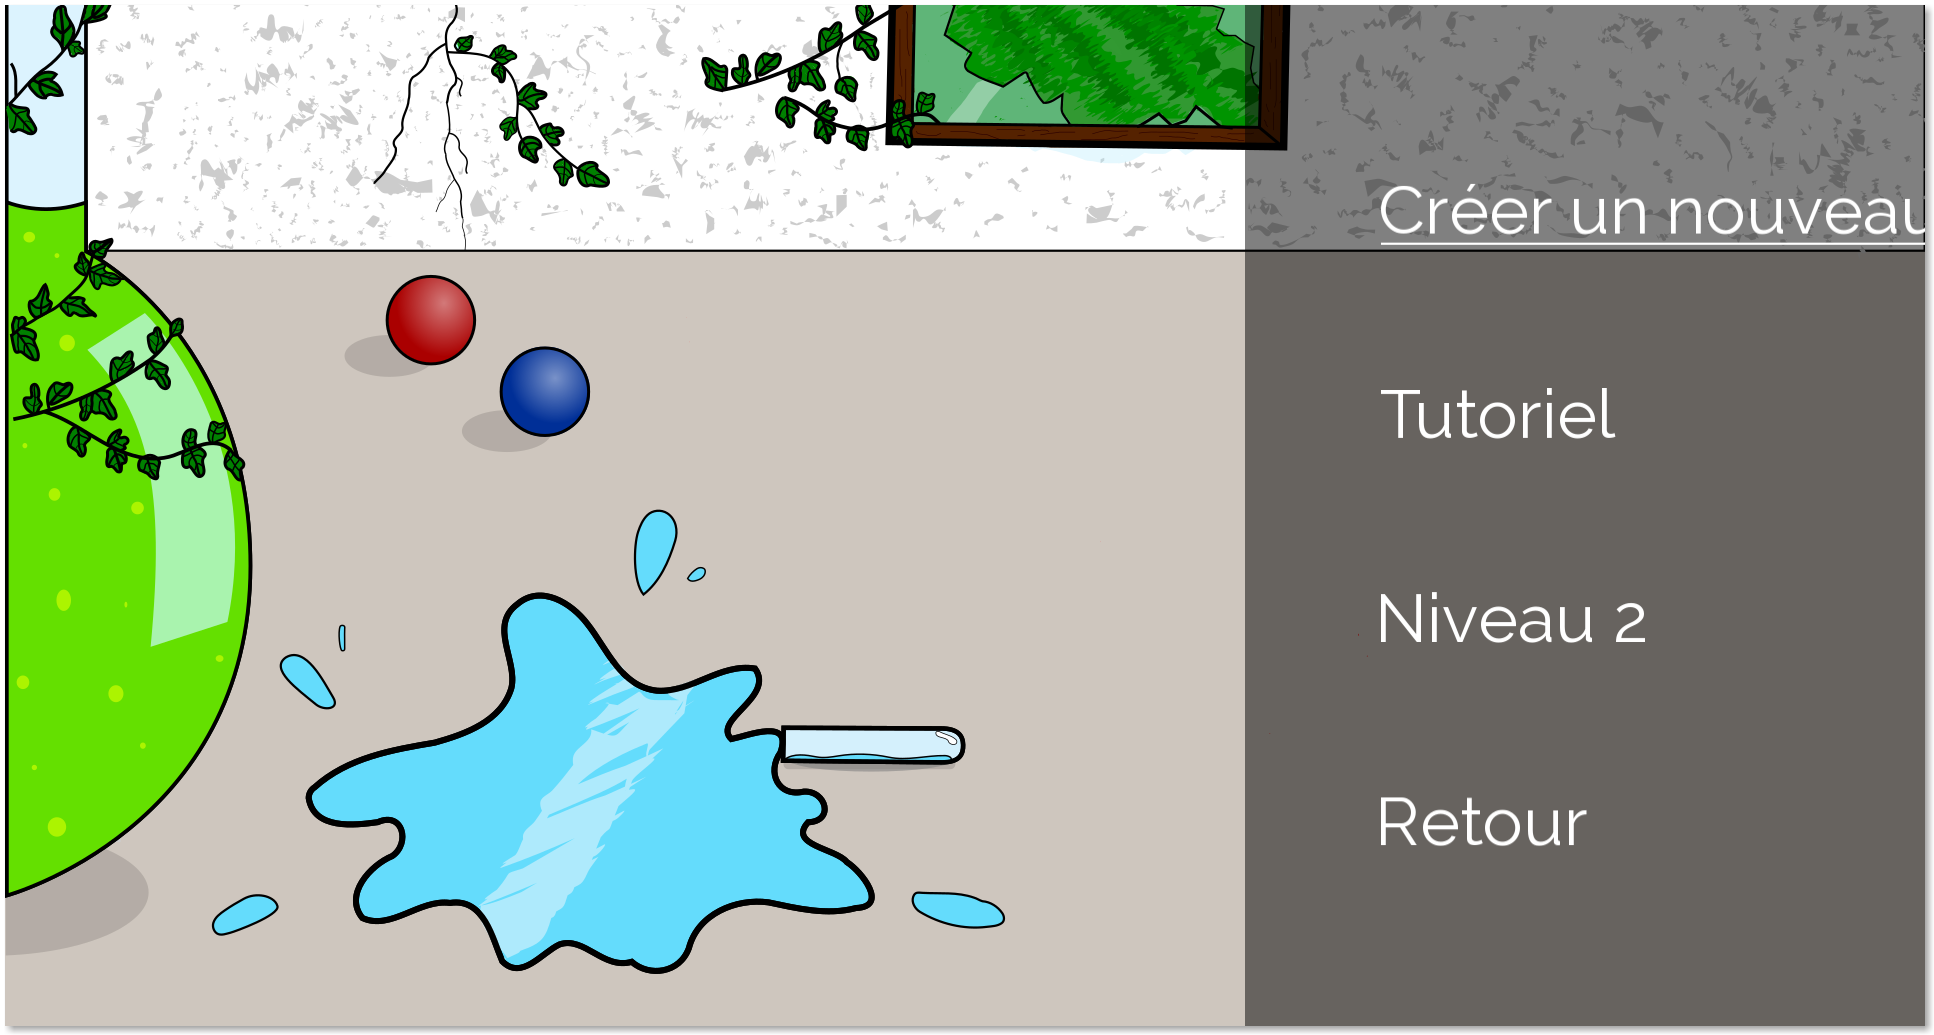
\includegraphics[width=13cm]{figures/menu_editeur.png}}
    \caption {Menu éditeur}
    \label {fig:ME}
\end{figure}


\noindent Ce menu [\ref{fig:ME}] se compose de trois types de boutons : Créer un nouveau niveau, éditer un niveau existant,
 et retour qui renvoie vers le menu principal [\ref{fig:MP}].\\




\noindent Les touches \Touche{$\uparrow$} , \Touche{$\downarrow$} ou
le passage de la souris sur un des boutons permettent la séléction d'un élément du menu.
le bouton sélectionné se souligne.\\

\noindent La touche \Touche{Enter} ou un clic avec la souris permettent de valider le choix.\\

\noindent Les touches \Touche{Backspace} et \Touche{Echap} permettent de revenir au menu précédent. \\

\subsection {Objets}

\label {OB}

\subsubsection{Balles}

\noindent {\raisebox{-.4\height}{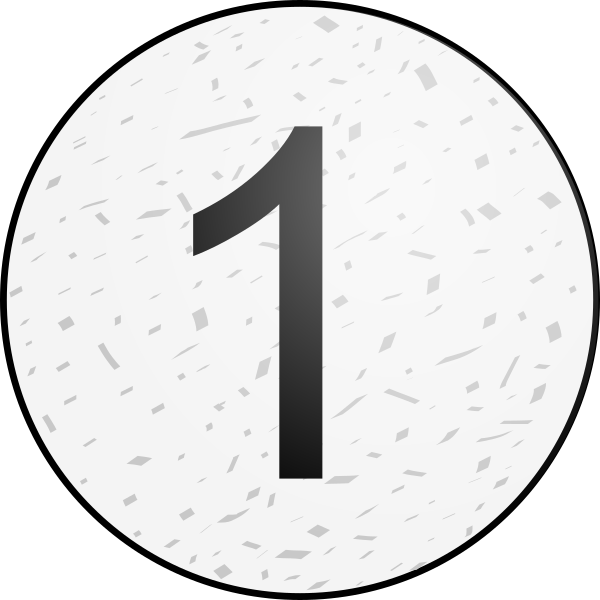
\includegraphics[width=23px]{figures/ball_1.png}} Les balles sont controlées par les joueurs. \\

\subsubsection{Polarité}

\noindent {\raisebox{-.4\height}{
\includegraphics[width=23px]{figures/block_blue.png}} Les objets de couleurs bleus repoussent tous ceux de la même couleur et attirent les objets de couleurs rouges. \\

\noindent {\raisebox{-.4\height}{
\includegraphics[width=23px]{figures/block_red.png}} Les objets de couleurs rouges repoussent tous ceux de la même couleur et attirent les objets de couleurs bleus. \\

\subsubsection{Blocs}

\noindent {\raisebox{-.4\height}{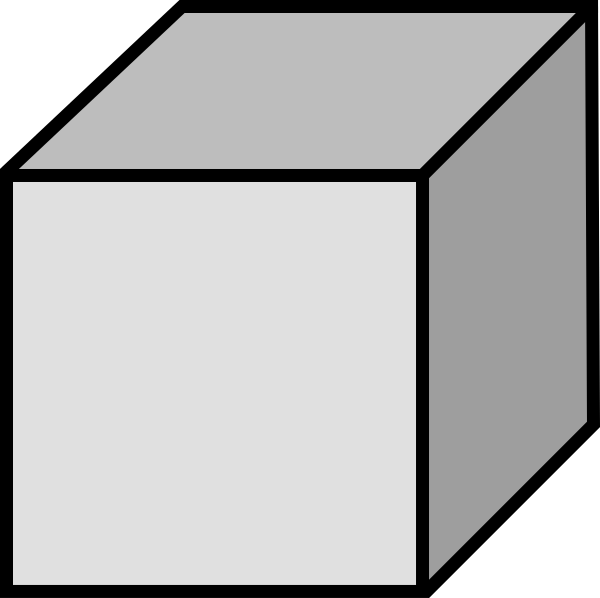
\includegraphics[width=23px]{figures/block.png}} Le bloc de base ne réalise aucune action particulière. \\

\noindent \raisebox{-.4\height}{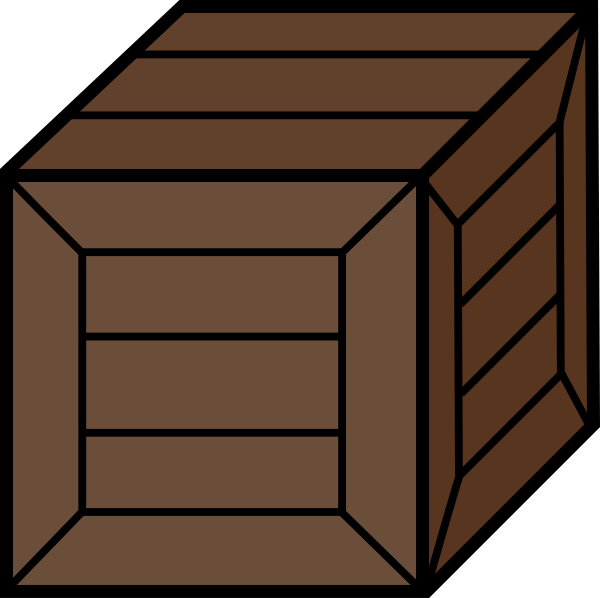
\includegraphics[width=23px]{figures/block_caisse.png}} La caisse est un bloc qui peut être poussé. \\

\noindent \raisebox{-.4\height}{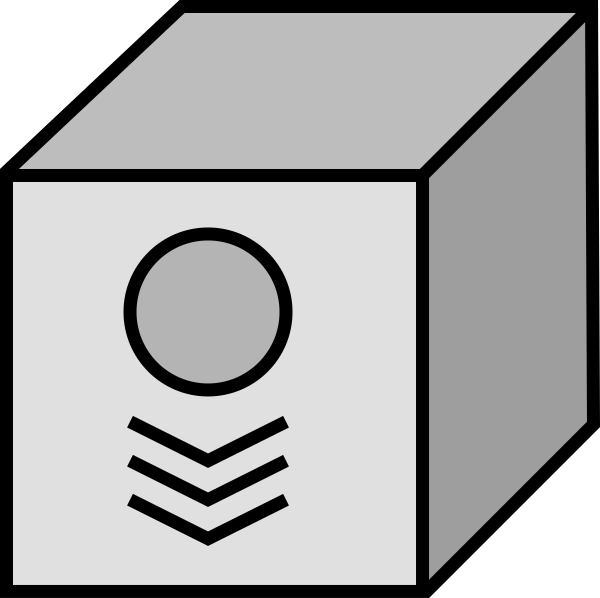
\includegraphics[width=23px]{figures/block_gravity_south.png}} Le bloc de gravité modifie le sens de la gravité lorsqu'un joueur ou une caisse rentre en collision avec lui. \\

\noindent \raisebox{-.4\height}{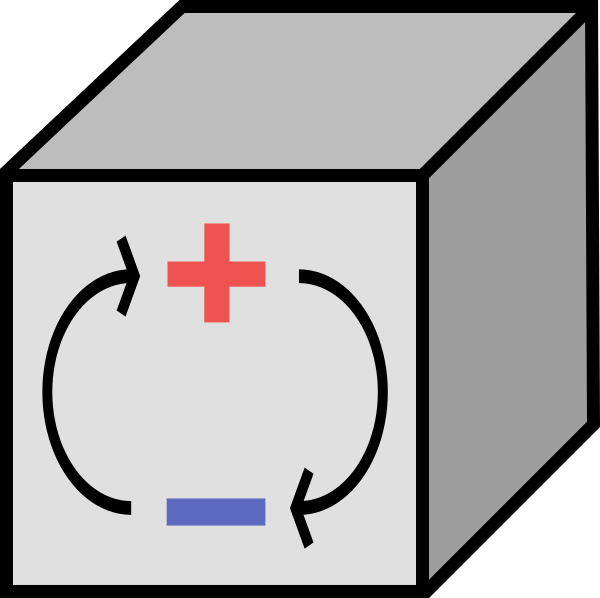
\includegraphics[width=23px]{figures/block_polarity.png}} Le bloc inverseur de polarité inverse la polarité de la balle qui rentre en collision avec lui. \\

\noindent \raisebox{-.4\height}{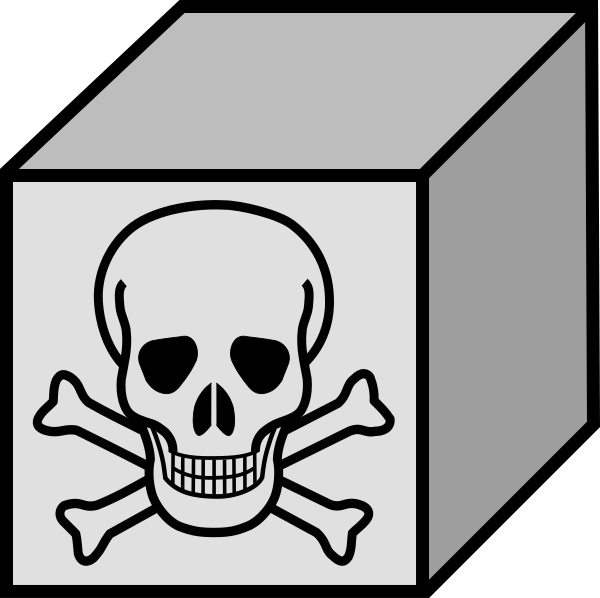
\includegraphics[width=23px]{figures/block_dead.png}} Le bloc de mort fait perdre la partie si un des deux joueurs rentrent en collision avec lui. \\

\noindent \raisebox{-.3\height}{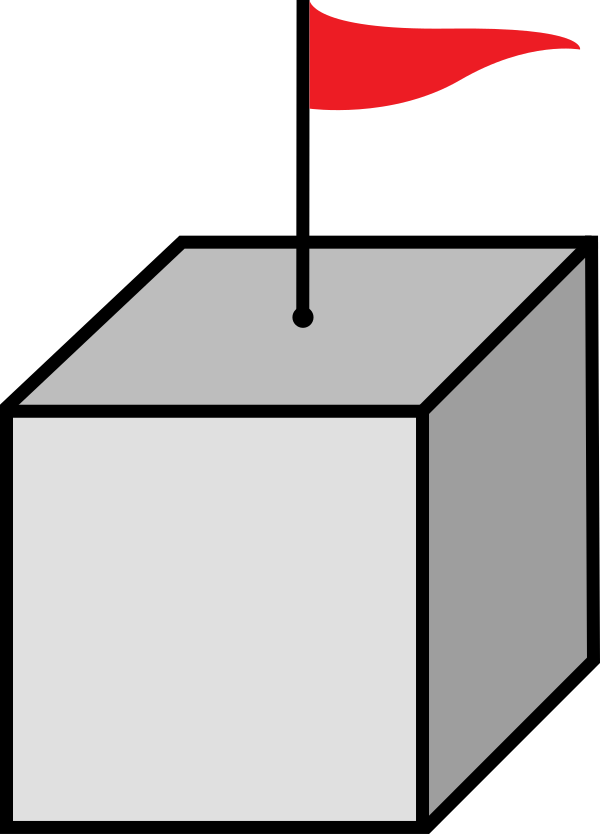
\includegraphics[width=23px]{figures/block_end_2.png}} Le bloc d'arrivée fait gagner le joueur qui rentre en collision avec lui. \\


\subsection {Jeux}

\label {joué}

Les joueurs ne peuvent déplacer leurs balles que vers la gauche ou la droite.\\
Le joueur 1 utilise \Touche{$\rightarrow$} pour se déplacer vers la droite et \Touche{$\leftarrow$} pour se déplacer vers la gauche.\\
Le joueur 2 utilise \Touche{D} pour se déplacer vers la droite et \Touche{Q} pour se déplacer vers la gauche.\\

Les joueurs peuvent mettre le jeu en pause avec la touche \Touche{Échap}, ou bien quitter le niveau en appuyant sur \Touche{Espace}.

Un joueur peut mourrir de deux façons; soit en rentrant en collision avec un bloc de mort \raisebox{-.4\height}{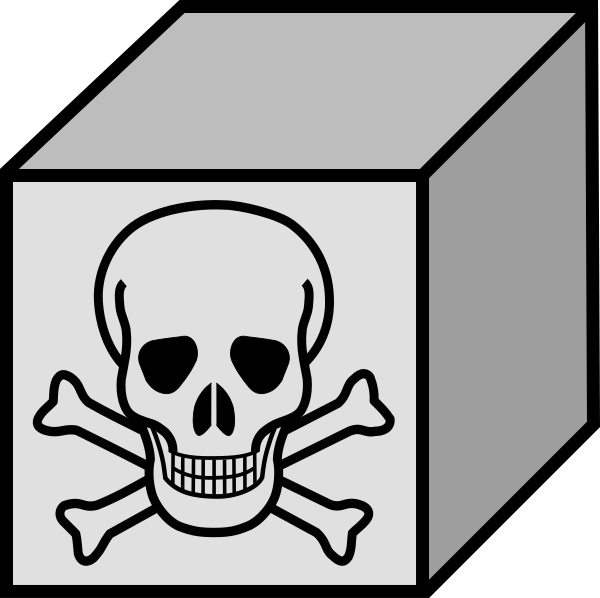
\includegraphics[width=15px]{figures/block_dead.png}} soit en sortant de la zone jouable.\\
\\

\subsection {Editeur}

\begin{figure} [!h]
    \centerline {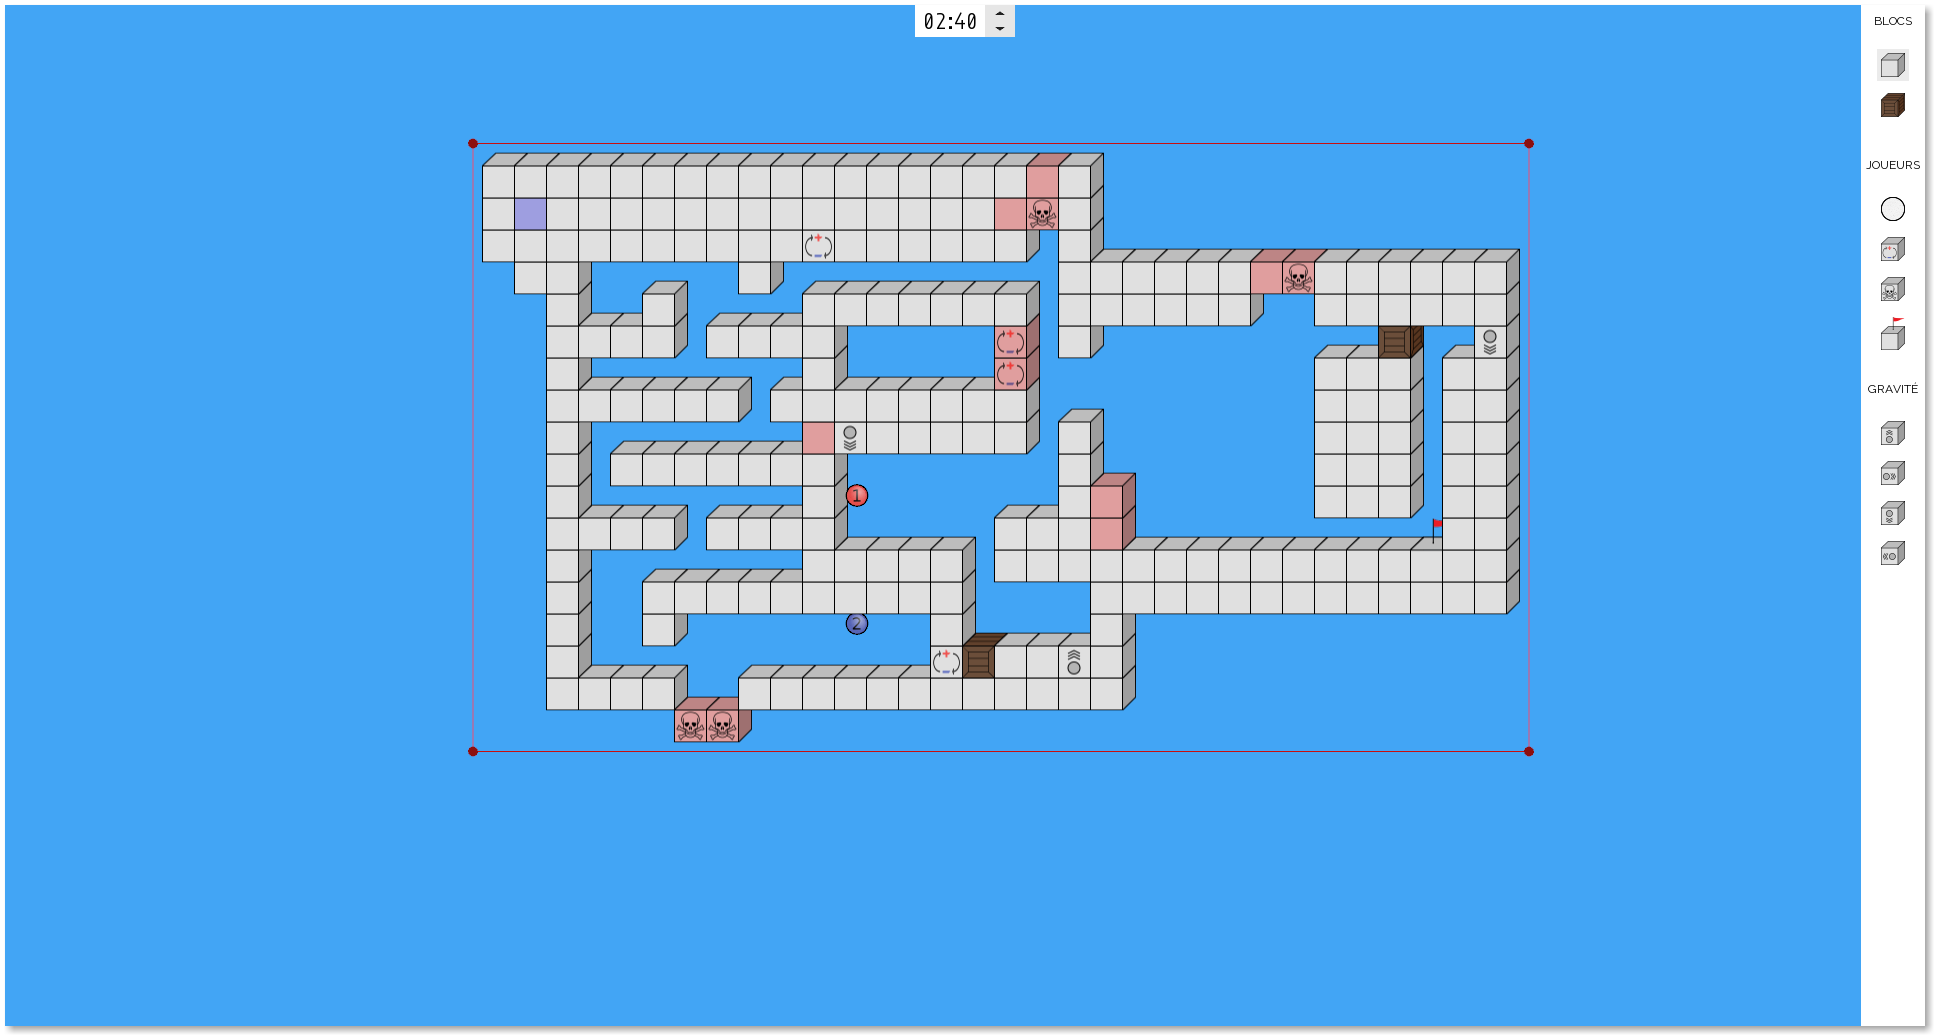
\includegraphics[width=13cm]{figures/editeur.png}}
    \caption {Éditeur}
    \label {fig:ED}
\end{figure}

\subsubsection {Gestion des objets}

La séléction de l'objet s'éffectue dans la barre latérale droite de la fenêtre à l'aide de la souris. [\ref{fig:ED}] \\
Un clic avec le bouton gauche de la souris permet de le placer sur un zone libre.
Le maintien du clic gauche permet de placer plusieurs objets à la fois.\\

Pour modifier la polarité d'un objet, le curseur doit être placé sur celui-ci. La touche \Touche{Ctrl} doit être enfoncée tout en faisant glisser la mollette de la souris, ou bien en faisant glisser deux doigts sur le pavé tactile vers le haut ou le bas. \\
\\

La selection d'un objet se fait avec la touche \Touche{Ctrl} et un clic sur celui-ci. Une multi-sélection peut être réalisée en cliquant sur plusieurs objets tout en maintenant la touche \Touche{Ctrl} enfoncée. \\
La réalisation d'une sélection rectangulaire est possible en maintenant la touche \Touche{Shift} et en faisant glisser la souris avec le clic gauche enfoncé sur la zone à sélectionner. \\
Un objet sélectionné a des bordures rouges. [\ref{fig:BBS}]\\

\begin{figure} [!h]
    \centerline {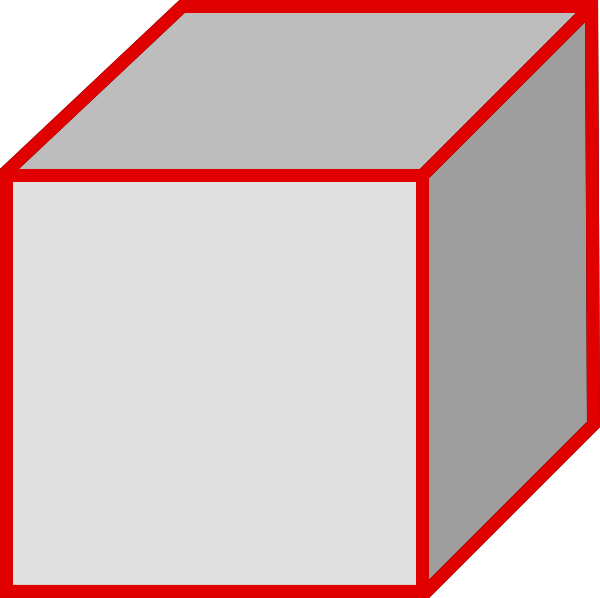
\includegraphics[width=25px]{figures/block_selection.png}}
    \caption {Bloc de base sélectionné}
    \label {fig:BBS}
\end{figure}

La suppression d'un objet s'effectue en cliquant dessus avec le bouton droit de la souris.
Plusieurs objets peuvent être supprimés aprés leurs séléctions en appuyant sur la touche \Touche{Suppr}.


\subsubsection {Compte à rebours}

Le compte à rebours se situe en haut au centre de le fenêtre. Durant la partie s'il arrive à 0, les joueurs meurent et la partie est perdue.\\

La valeur du compte à rebours peut être modifiée dans l'éditeur en cliquant sur les fléches se situant à coté.
Il est également possible de placer la souris sur ce dernier en faisant glisser la mollette ou deux doigts sur le pavé tactile vers le haut ou le bas. \\

\subsubsection {Zone de jeu}
La zone jouable est représentée dans l'éditeur par un polygone rouge [\ref{fig:ED}] composé de quatre points.
 Chacun de ces points peuvent être déplacés en cliquant dessus afin de modifier la taille et la forme de la zone.

\subsubsection {Gestion de la caméra}
Le déplacement de la caméra s'effectue en plaçant la souris vers une bordure de la fenêtre.
La molette de la souris peut être utilisée pour un défilement vertical ou horizontal si la touche \Touche{Shift} est enfoncée.
\\

il es possible également de faire glisser deux doigts sur le pavé tactile afin de déplacer la caméra dans la direction désirée.\\

\subsubsection {Commandes générales}

Il est possible de tester le niveau à tout moment en appuyant sur la touche \Touche{Espace}.
Pour revenir à l'édition il faut appuyer de nouveau sur \Touche{Espace}.\\
\\

Afin de sauvegarder le niveau il est necessaire de réaliser la combinaison de touches suivantes : \Touche{Ctrl} + \Touche {S}. (en mode édition).\\
\\

Pour quitter l’éditeur et revenir au menu la touche \Touche{Échap} doit être utilisé.
